% Created 2021-12-15 mié 23:15
% Intended LaTeX compiler: lualatex
\documentclass{IEEEtran}
\usepackage[left=1.5cm,right=1.5cm,letterpaper]{geometry}
\usepackage[spanish, es-nodecimaldot, es-tabla]{babel}
\usepackage[utf8]{inputenc}
\usepackage{blindtext}
\usepackage{subfigure}
\usepackage[most]{tcolorbox}
\usepackage{etoolbox}
\usepackage{minted}
\usepackage{hyperref}
\usepackage{xcolor}
\definecolor{LightGray}{gray}{0.9}
\definecolor{DarkGray}{HTML}{191919}
\definecolor{custom}{HTML}{FFFFFF}
\usepackage{caption}
\usemintedstyle{emacs}
\usepackage[ruled,vlined]{algorithm2e}
\newenvironment{code}{\captionsetup{type=listing}}{}
\setminted{frame=lines,breaklines=true,fontsize=\scriptsize,autogobble}
\renewcommand{\listingscaption}{Código}
\renewcommand\listoflistingscaption{Índice de \listingscaption\@s}
\BeforeBeginEnvironment{minted}{\begin{code}}
\AfterEndEnvironment{minted}{\end{code}}
\usepackage[backend=biber,style=ieee]{biblatex}
\addbibresource{./main.bib}
\author{Castelan Hernandez Mario, Miranda Hernández Alejandro, Romero Andrade Cristian, Sánchez Brito Diego y Solano Morales Isaac Uriel}
\date{\today}
\title{Proyecto - Organización y Arquitectura de Computadoras}
\hypersetup{
 pdfauthor={Castelan Hernandez Mario, Miranda Hernández Alejandro, Romero Andrade Cristian, Sánchez Brito Diego y Solano Morales Isaac Uriel},
 pdftitle={Proyecto - Organización y Arquitectura de Computadoras},
 pdfkeywords={},
 pdfsubject={},
 pdfcreator={Emacs 27.2 (Org mode 9.6)}, 
 pdflang={Spanish}}
\begin{document}

\begin{titlepage}
\centering
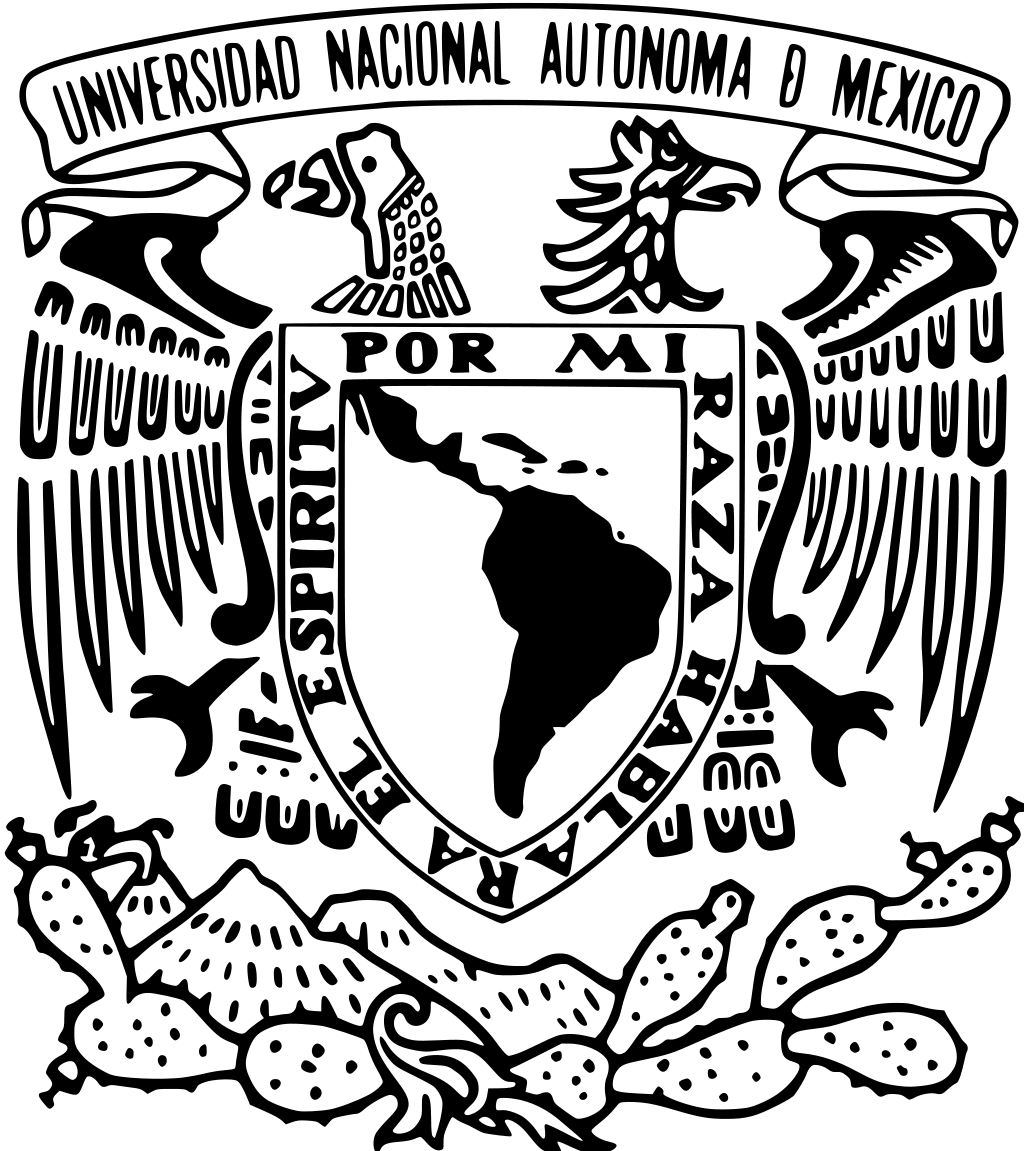
\includegraphics[width=0.25\textwidth]{./img_common/unam_logo}\vspace{0.5cm}\\
{\scshape{\Huge Facultad de Ingeniería\par{}}}\vspace{0.25cm}
{\scshape{\Large Organización y Arquitectura de Computadoras\par{}}}\vfill{}
{\huge \textbf{Proyecto de Organización y Arquitectura de Computadoras}}\vfill{}
{\Large Alumnos\\
Castelan Hernandez Mario

Miranda Hernández Alejandro

Romero Andrade Cristian

Sánchez Brito Diego

Solano Morales Isaac Uriel

}\vfill{}
{\large Grupo: 01\par{}}\vfill{}
{\large Profesor\\Ing.~Hugo Enrique Estrada León}\vfill{}
\vfil{}
{\large Semestre\\\textbf{2022--1}}
\vfill{}
{\large Fecha de Entrega\\17 de diciembre de 2021}
\vfill{}

\includegraphics[width=0.1\textwidth]{./img_common/inge_logo}
\end{titlepage}

\maketitle
\tableofcontents

\section{Objetivo}
\label{sec:orgcf1df0f}
El alumno programará las instrucciones necesarias para poder ejecutar un algoritmo sobre una arquitectura de computadora  diseñada por el alumno.
\subsection{Algoritmos}
\label{sec:org731bfb7}
Se debe elegir alguno de los algoritmos propuestos e implementar la o las instrucciones necesarias para llevarlo a cabo. Los modos de direccionamiento y la arquitectura son libres de elección.
Si se elige la arquitectura RISC, se tendrá un pontaje extra en la calificación. En
dado caso que para su algoritmo existan riesgos por dependencia de datos, estos
se solucionarían vía software (agregando instrucciones \texttt{NOP}) y no por hardware.
\subsection{Área de un octágono}
\label{sec:org87b5c07}
Se debe implementar el algoritmo que permita obtener el área de un octágono. Se usará la siguiente formula:
\(A = \frac{perimetro \times apotema}{2}\)
siendo el \(perimetro\) y el \(apotema\) números enteros.
\section{Introducción}
\label{sec:org44245a3}
\subsection{Arquitectura y organización de la computadora}
\label{sec:org6d70538}
La arquitectura de la computadora hace referencia al conjunto de elementos del computador que son visibles desde el punto de vista del programador de ensamblador.
La organización de la computadora se refiere a las unidades funcionales del computador y al modo como están interconectadas.
\subsection{Arquitectura Von Neumann}
\label{sec:org770d39e}
El objetivo de la arquitectura Von Neumann es construir un sistema flexible que permita resolver diferentes tipos de problemas. Para conseguir esta flexibilidad, se construye un sistema de propósito general que se pueda programar para resolver los diferentes tipos de problemas. Para cada problema concreto se define un programa diferente.
La arquitectura Von Neumann se basa en tres propiedades:
\begin{enumerate}
\item Hay un único espacio de memoria de lectura y escritura, que contiene las instrucciones y los datos necesarios.
\item El contenido de la memoria es accesible por posición, independientemente de que se acceda a datos o a instrucciones.
\item La ejecución de las instrucciones se produce de manera secuencial: después de ejecutar una instrucción se ejecuta la instrucción siguiente que hay en la memoria principal, pero se puede romper la secuencia de ejecución utilizando instrucciones de ruptura de secuencia.
\end{enumerate}
\subsection{Arquitectura Harvard}
\label{sec:org985add2}
La organización del computador según el modelo Harvard, básicamente, se distingue del modelo Von Neumann por la división de la memoria en una memoria de instrucciones y una memoria de datos, de manera que el procesador puede acceder separada y simultáneamente a las dos memorias.
\begin{figure}[htbp]
\centering
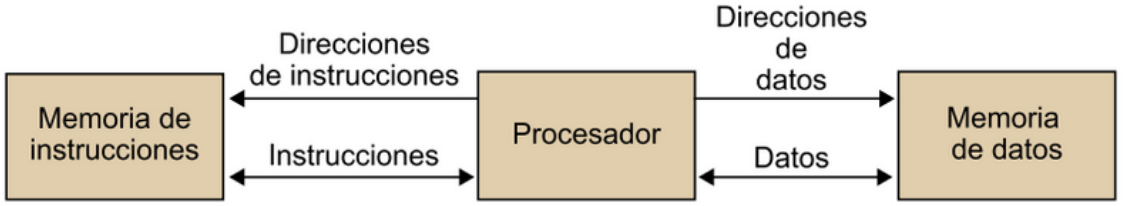
\includegraphics[width=.9\linewidth]{./img/arq_harv.png}
\caption{Arquitectura Harvard}
\end{figure}
\subsection{RISC: Reduced instruction set computer processor}
\label{sec:orgec51ecd}
Es una arquitectura de procesadores basada en una colección de instrucciones simples y altamente personalizadas. RISC se construye para minimizar el tiempo de ejecución de una instrucción, optimizando y limitando el número de instrucciones. La arquitectura RISC tiene la capacidad de por cada ciclo de instrucción se da solo un ciclo de reloj. Cada ciclo debe contener cuatro etapas: buscar, decodificar, ejecutar y guardar.
\subsection{CISC: complex instruction set computer}
\label{sec:org6dfac74}
CISC es un sistema de instrucciones desarrollado por Intel que requieren de mucho tiempo para ser ejecutadas completamente.
Lo que sucede en CISC es que se reduce la cantidad de instrucciones de un software y se ignora el número de ciclos por instrucción. Se especializa en crear instrucciones complejas en el hardware, ya que el hardware siempre será mucho más rápido que el software.
\section{Desarrollo}
\label{sec:orgca6fb84}
Primeramente se diseñan las etapas de la arquitectura RISC, las cuales se dividen en cuatro:
\begin{enumerate}
\item Llamada a la instrucción
\item Decodificación de la Instrucción
\item Llamada a los operadores
\item Ejecución
\end{enumerate}

Para la arquitectura 68HC11 cada instrucción ejecuta los siguientes pasos:
\begin{enumerate}
\item Obtener instrucción ejecutable de la memoria (bucle de recuperación)
\item Instrucciones de decodificación
\item Si la instrucción solicita leer un operando de la memoria, entonces se calcula la dirección efectiva de ese operando y los datos se leen de la memoria.
\item Si lo requiere la instrucción, los operandos requeridos se leen de los registros internos del microprocesador.
\item Ejecución, es decir, la operación se realiza en un bloque de procesamiento aritmético con operandos leídos previamente
\item Los resultados de la operación se guardan y el registro de banderas se actualiza
\end{enumerate}

Se ve que los pasos son similares a los ejecutados en las cartas ASM para las instrucciones. La arquitectura segmentada 68HC11 también realiza los mismos pasos, pero se agrupará en los siguientes cuatro pasos
\begin{enumerate}
\item Etapa IF (instruction fetch). La instrucción a ejecutar es leída de la memoria de instrucciones
\item Etapa ID (instruction decode). Se decodifica la instrucción y se traen los operandos necesarios por la instrucción (tanto de memoria como de registros internos)
\item Etapa EX (execution). Se procesan los operandos en la UPA (unidad de procesos aritméticos)
\item Etapa WB (write back). Se guardan resultados
\end{enumerate}
\begin{figure}[htbp]
\centering
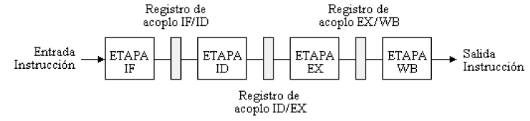
\includegraphics[width=.9\linewidth]{./img/etapas.png}
\caption{Etapas para la arquitectura segmentada del 68HC11}
\end{figure}
\subsection{Etapa 1}
\label{sec:org69a78c2}
En esta etapa tenemos contadores, incrementadores, multiplexores y memoria de instrucciones conectados entre sí \cite[p, 133]{SAVAGE}, arrojando su salida al registro de la PC y las instrucciones que serán tomadas posteriormente por la etapa 2.
\begin{center}
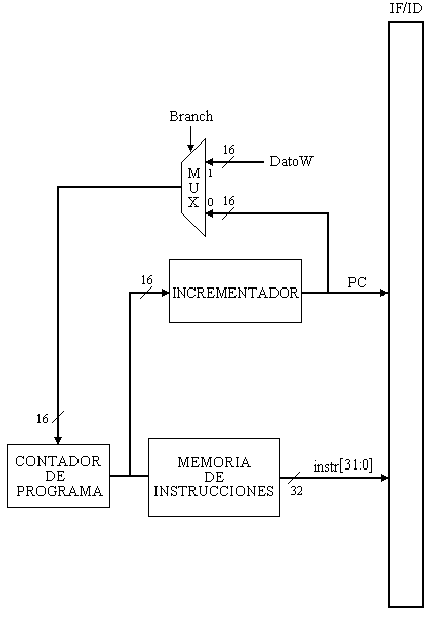
\includegraphics[width=0.6\linewidth]{./img/e1s.png}
\captionof{figure}{Etapa 1 \cite[p, 133]{SAVAGE}}
\end{center}
\begin{figure}[htbp]
\centering
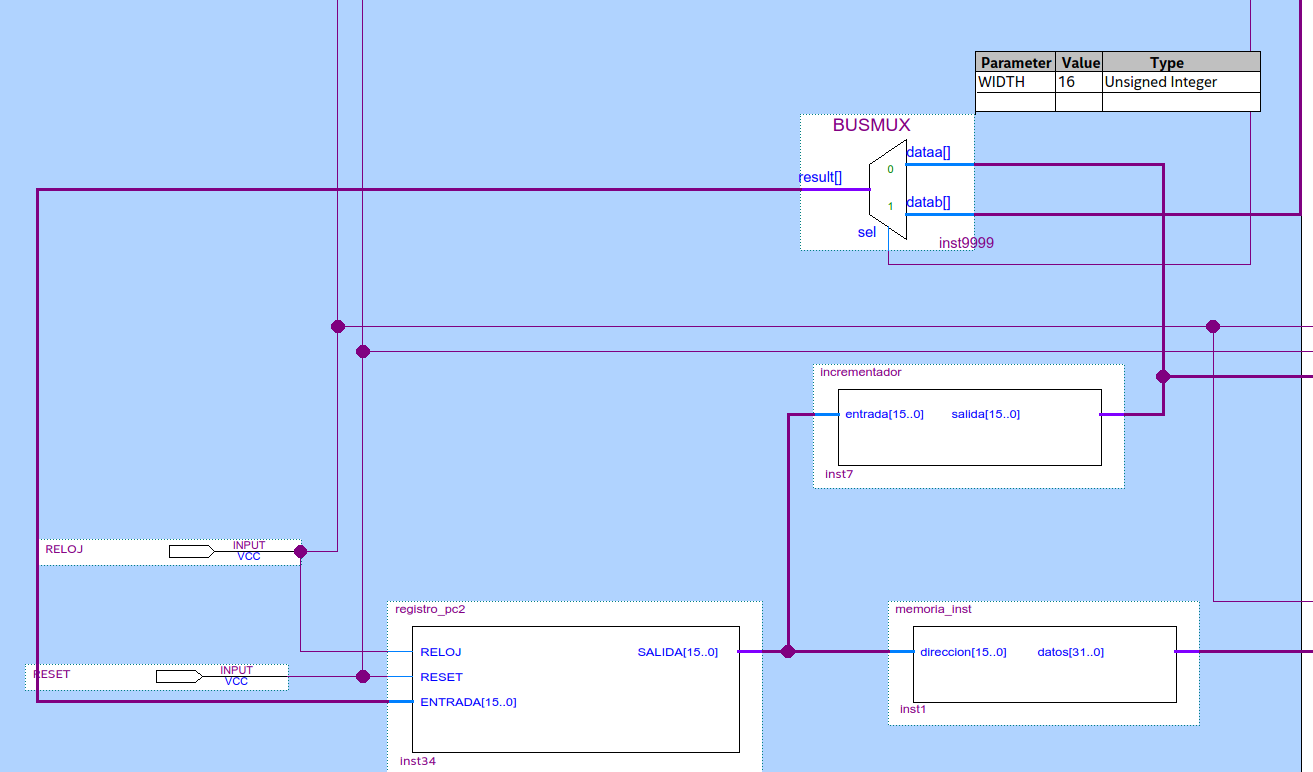
\includegraphics[width=.9\linewidth]{./img/e1.png}
\caption{Etapa 1}
\end{figure}
\subsection{Etapa 2}
\label{sec:org6205604}
Luego tenemos la etapa 2 con los bloques que se muestran en la introducción, destacando los registros internos básicos, módulos de control, sumadores y registros de acoplamiento para
poder ejecutar el pipeline, teniendo sus respectivas salidas para poder hacerlo\footnote{Se recomienda apreciar la arquitectura en Quartus descargando el proyecto como se explica en la \hyperref[sec:instalacion]{seccion instalación}.}.
\begin{center}
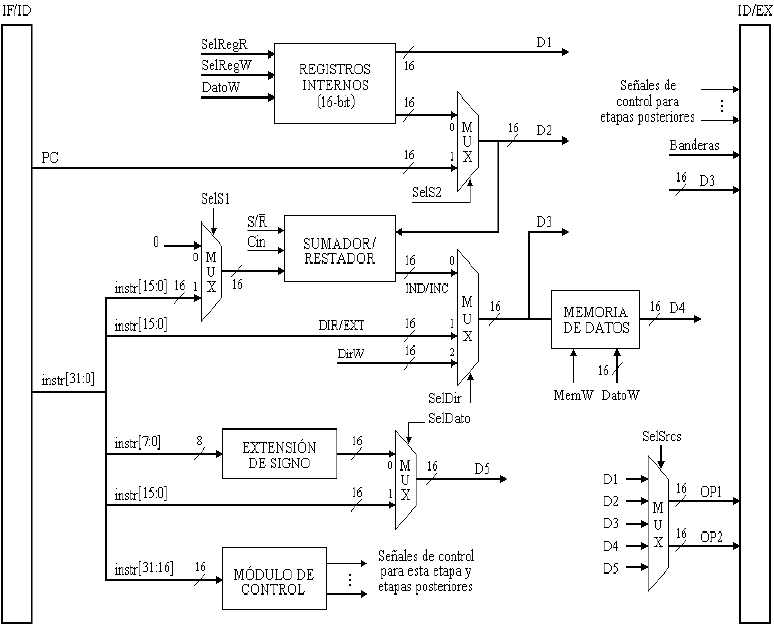
\includegraphics[width=\linewidth]{./img/e2s.png}
\captionof{figure}{Etapa 2 \cite[p, 135]{SAVAGE}}
\end{center}
\begin{figure}[htbp]
\centering
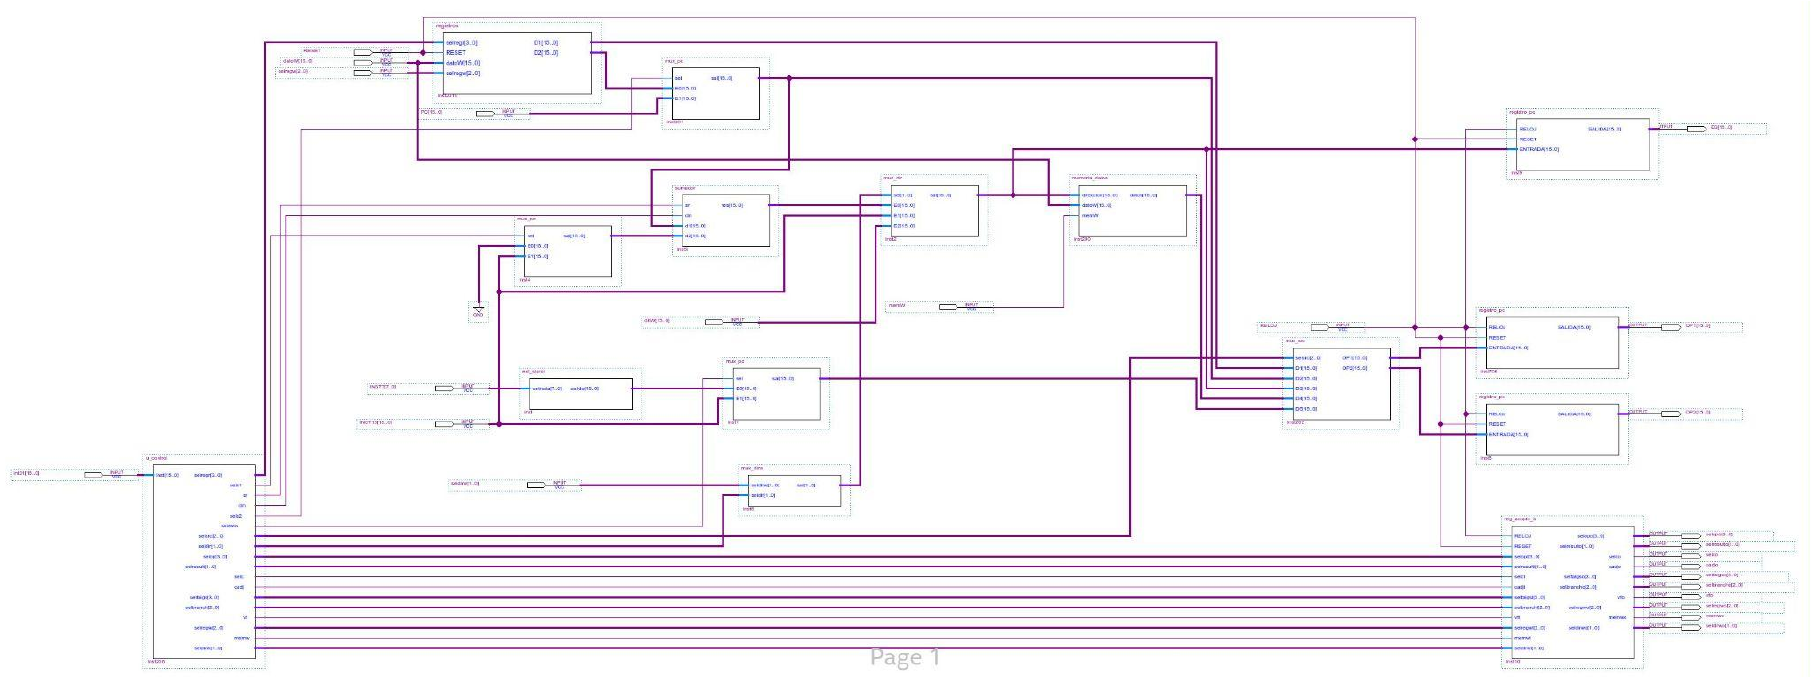
\includegraphics[width=.9\linewidth]{./img/e2.png}
\caption{Etapa 2}
\end{figure}
\subsection{Etapa 3}
\label{sec:orge6aad5b}
Finalmente, la etapa 03\footnote{Ya que la etapa 04 es solo una salida o las banderas que se activan durante todo el proceso}, lo cual se hace directamente para poder simularlo de una buena manera en vhdl.
Como podemos ver en esta etapa 03 tenemos la UPA y el generador de banderas, los cuales se muestran de forma independiente, cada uno con su bloque para poder controlarlo de mejor manera y poder mostrarlo en la simulación
\begin{center}
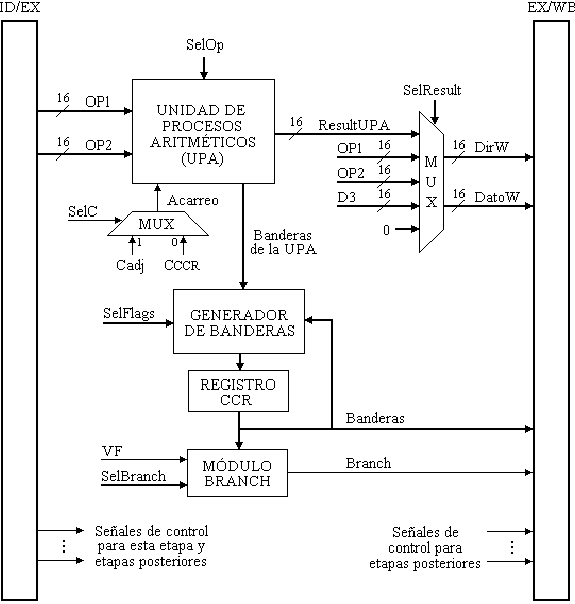
\includegraphics[width=\linewidth]{./img/e3s.png}
\captionof{figure}{Etapa 3 \cite[p, 139]{SAVAGE}}
\end{center}
\begin{figure}[htbp]
\centering
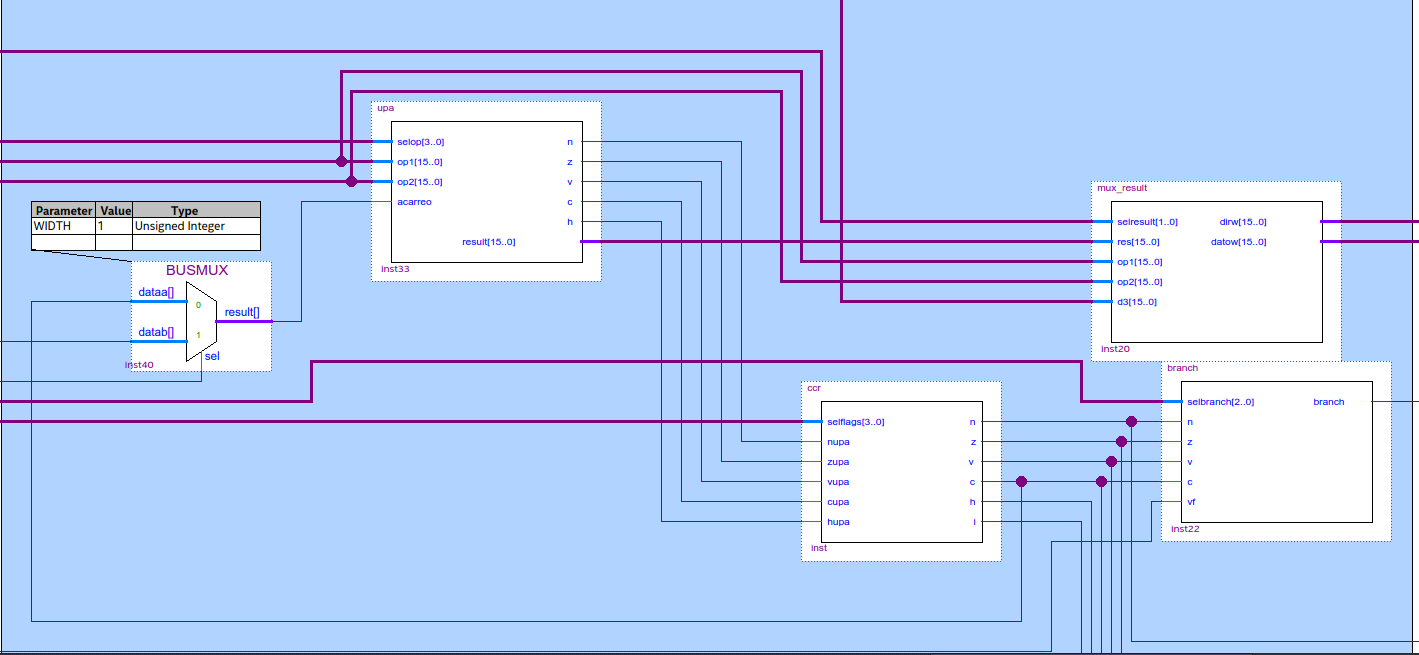
\includegraphics[width=.9\linewidth]{./img/e3.png}
\caption{Etapa 3}
\end{figure}
\begin{center}
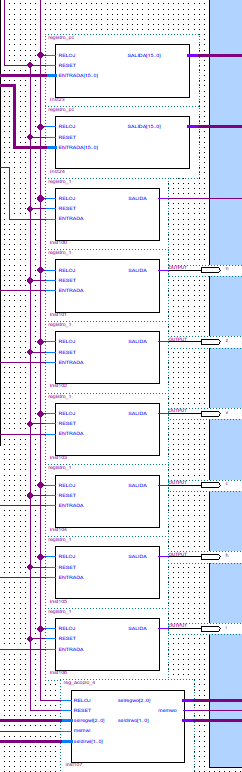
\includegraphics[width=0.5\linewidth]{./img/e4.png}
\captionof{figure}{Etapa 4}
\end{center}

\subsection{Resolución del algoritmo}
\label{sec:org6bf37e7}
Primeramente definimos el problema, es la división entre 2 de el producto de dos números.
\subsubsection{División}
\label{sec:org116026f}
La división se puede simular haciendo que se recorra un bit a la derecha, por lo tanto, basándonos del set de instrucciones la instrucción perfecta es \texttt{ASRB}\footnote{Notación Mnemónico.} (\(0057\)\footnote{Instrucción.}) \cite[p. 24]{PM1999}, podemos implementarlo en RISC definiendo las siguientes señales de control:
\begin{table}[htbp]
\caption{Señales de control de \texttt{ASRB} (\(0057\))}
\centering
\begin{tabular}{ll}
\hline
selregr & \texttt{5}\\
sels1 & \texttt{0}\\
sr & \texttt{1}\\
cin & \texttt{0}\\
sels2 & \texttt{0}\\
seldato & \texttt{1}\\
selsrc & \texttt{1}\\
seldir & \texttt{0}\\
selop & \texttt{7}\\
selresult & \texttt{1}\\
selc & \texttt{1}\\
cadj & \texttt{0}\\
selfalgs & \texttt{3}\\
selbranch & \texttt{0}\\
vf & \texttt{1}\\
selregw & \texttt{4}\\
memw & \texttt{0}\\
seldirw & \texttt{0}\\
\hline
\end{tabular}
\end{table}
Por lo tanto, el fragmento en el archivo \texttt{u\_control.vhd} seria el siguiente:
\begin{code}
\caption{\texttt{ASRB} en \texttt{u\_control.vhd}}
\inputminted[firstline=413, lastline=431]{vhdl}{../Risc/u_control.vhd}
\end{code}
\subsubsection{Multiplicación}
\label{sec:org2da015f}
Tenemos dos opciones:, 1) realizar el módulo de multiplicación para la arquitectura en RISC y 2) realizar la multiplicación usando software. Se optó por usar software, por lo tanto definimos nuestro algoritmo en la cual nos basaremos para implementarlo en ensamblador y después pasarlo a memoria.
\begin{algorithm}
\caption{Algoritmo de multiplicación propuesto}
\KwResult{$perimetro \times apotema$}
$a \gets perimetro$\;
$b \gets apotema$\;
$suma\_auxiliar \gets a$\;
$i \gets 0$\;
\While{$i \neq b$}{
  $suma\_auxiliar \gets suma\_auxiliar \times a$\;
  $i \gets i + 1$\;
}
\end{algorithm}
Teniendo este punto resuelto buscamos que instrucciones nos pueden servir\cite[pp. 24-26]{PM1999}:
\begin{itemize}
\item \texttt{LDAA}
\begin{itemize}
\item Acceso Inmediato: Carga en el registro ACCA un dato inmediato de 16 bits contenido en memoria.
\item Acceso Directo: Carga en el acumulador A, un dato inmediato de 8 bits contenido en memoria.
\end{itemize}
\begin{table}[htbp]
\caption{LDAA}
\centering
\begin{tabular}{lll}
\hline
 & Acceso & Acceso\\
 & Inmediato (\(0086\)) & Directo (\(0096\))\\
\hline
selregr & \texttt{0} & \texttt{0}\\
sels1 & \texttt{0} & \texttt{0}\\
sr & \texttt{1} & \texttt{1}\\
cin & \texttt{0} & \texttt{0}\\
sels2 & \texttt{0} & \texttt{0}\\
seldato & \texttt{1} & \texttt{1}\\
selsrc & \texttt{3} & \texttt{2}\\
seldir & \texttt{0} & \texttt{1}\\
selop & \texttt{4} & \texttt{4}\\
selresult & \texttt{1} & \texttt{1}\\
selc & \texttt{1} & \texttt{1}\\
cadj & \texttt{0} & \texttt{0}\\
selfalgs & \texttt{1} & \texttt{1}\\
selbranch & \texttt{0} & \texttt{0}\\
vf & \texttt{1} & \texttt{1}\\
selregw & \texttt{1} & \texttt{1}\\
memw & \texttt{0} & \texttt{0}\\
seldirw & \texttt{0} & \texttt{0}\\
\hline
\end{tabular}
\end{table}
\end{itemize}
\begin{code}
\caption{\texttt{LDAA} de acceso inmediato en \texttt{u\_control.vhd}}
\inputminted[firstline=53, lastline=71]{vhdl}{../Risc/u_control.vhd}
\end{code}
\begin{code}
\caption{\texttt{LDAA} de acceso directo en \texttt{u\_control.vhd}}
\inputminted[firstline=93, lastline=111]{vhdl}{../Risc/u_control.vhd}
\end{code}
\begin{itemize}
\item \texttt{STAA}
Suma los contenidos de los registros acumuladores A y B. El resultado es guardado en el acumulador A.
\begin{table}[htbp]
\caption{\texttt{STAA} (\(00B7\))}
\centering
\begin{tabular}{ll}
\hline
selregr & \texttt{4}\\
sels1 & \texttt{1}\\
sr & \texttt{1}\\
cin & \texttt{0}\\
sels2 & \texttt{0}\\
seldato & \texttt{1}\\
selsrc & \texttt{1}\\
seldir & \texttt{0}\\
selop & \texttt{4}\\
selresult & \texttt{1}\\
selc & \texttt{1}\\
cadj & \texttt{0}\\
selfalgs & \texttt{1}\\
selbranch & \texttt{0}\\
vf & \texttt{1}\\
selregw & \texttt{0}\\
memw & \texttt{1}\\
seldirw & \texttt{2}\\
\hline
\end{tabular}
\end{table}
\end{itemize}
\begin{code}
\caption{\texttt{STAA} en \texttt{u\_control.vhd}}
\inputminted[firstline=133, lastline=151]{vhdl}{../Risc/u_control.vhd}
\end{code}
\begin{itemize}
\item \texttt{LDAB}
\begin{itemize}
\item Acceso Inmediato: Carga en el registro ACCB un dato inmediato de 16 bits contenido en memoria.
\item Acceso Directo: Carga en el acumulador B, un dato inmediato de 8 bits contenido en memoria.
\end{itemize}
\begin{table}[htbp]
\caption{\texttt{LDAB}}
\centering
\begin{tabular}{lll}
\hline
 & Acceso & Acceso\\
 & Inmediato (\(00C6\)) & Directo (\(00D6\))\\
\hline
selregr & \texttt{0} & \texttt{0}\\
sels1 & \texttt{0} & \texttt{0}\\
sr & \texttt{1} & \texttt{1}\\
cin & \texttt{0} & \texttt{0}\\
sels2 & \texttt{0} & \texttt{0}\\
seldato & \texttt{1} & \texttt{1}\\
selsrc & \texttt{3} & \texttt{2}\\
seldir & \texttt{0} & \texttt{1}\\
selop & \texttt{4} & \texttt{4}\\
selresult & \texttt{1} & \texttt{1}\\
selc & \texttt{1} & \texttt{1}\\
cadj & \texttt{0} & \texttt{0}\\
selfalgs & \texttt{1} & \texttt{1}\\
selbranch & \texttt{0} & \texttt{0}\\
vf & \texttt{1} & \texttt{1}\\
selregw & \texttt{4} & \texttt{4}\\
memw & \texttt{0} & \texttt{0}\\
seldirw & \texttt{0} & \texttt{0}\\
\hline
\end{tabular}
\end{table}
\begin{code}
\caption{\texttt{LDAB} de acceso inmediato en \texttt{u\_control.vhd}}
\inputminted[firstline=73, lastline=91]{vhdl}{../Risc/u_control.vhd}
\end{code}
\begin{code}
\caption{\texttt{LDAB} de acceso directo en \texttt{u\_control.vhd}}
\inputminted[firstline=113, lastline=131]{vhdl}{../Risc/u_control.vhd}
\end{code}
\item \texttt{CBA} (\(0011\))
Suma el acumulador A más el acumulador B y lo almacena en el acumulador A.
\begin{table}[htbp]
\caption{\texttt{CBA}}
\centering
\begin{tabular}{ll}
\hline
selregr & \texttt{1}\\
sels1 & \texttt{0}\\
sr & \texttt{1}\\
cin & \texttt{0}\\
sels2 & \texttt{0}\\
seldato & \texttt{1}\\
selsrc & \texttt{1}\\
seldir & \texttt{0}\\
selop & \texttt{2}\\
selresult & \texttt{0}\\
selc & \texttt{1}\\
cadj & \texttt{1}\\
selfalgs & \texttt{3}\\
selbranch & \texttt{0}\\
vf & \texttt{1}\\
selregw & \texttt{0}\\
memw & \texttt{0}\\
seldirw & \texttt{0}\\
\hline
\end{tabular}
\end{table}
\begin{code}
\caption{\texttt{CBA} en \texttt{u\_control.vhd}}
\inputminted[firstline=233, lastline=251]{vhdl}{../Risc/u_control.vhd}
\end{code}
\item \texttt{JMP} (\(007E\))
Salta a una instrucción de la memoria.
\begin{table}[htbp]
\caption{\texttt{JMP}}
\centering
\begin{tabular}{ll}
\hline
selregr & \texttt{126}\\
sels1 & \texttt{0}\\
sr & \texttt{0}\\
cin & \texttt{0}\\
sels2 & \texttt{1}\\
seldato & \texttt{1}\\
selsrc & \texttt{3}\\
seldir & \texttt{0}\\
selop & \texttt{4}\\
selresult & \texttt{1}\\
selc & \texttt{0}\\
cadj & \texttt{0}\\
selfalgs & \texttt{0}\\
selbranch & \texttt{0}\\
vf & \texttt{0}\\
selregw & \texttt{0}\\
memw & \texttt{0}\\
seldirw & \texttt{0}\\
\hline
\end{tabular}
\end{table}
\begin{code}
\caption{\texttt{CBA} en \texttt{u\_control.vhd}}
\inputminted[firstline=253, lastline=271]{vhdl}{../Risc/u_control.vhd}
\end{code}
\end{itemize}

\begin{code}
\caption{Pseudocódigo ensamblador que nos auxiliara para implementarlo en la memoria, se usa como entradas 6 y 2}
\begin{minted}[linenos,numbersep=1pt]{GAS}
ldaa 6 ; Valor de entrada A
staa 2
ldaa 8 ; Valor de entrada B
staa 3

ldaa 0 ; iterador
staa 0

ldaa 2 ; Auxiliar
staa 4

ldab 3 ; B

cba ; Si ACCB es diferente a ACCA, salta la siguiente instrucción, si no, se va a la instrucción 28
jmp 28

ldaa 4
ldab 2
aba
ldab 3
ldaa 4
ldaa 0
inca

staa 0
jmp 12

ldab 4
acrb
\end{minted}
\end{code}

Teniendo el código ensamblador de referencia escribimos en memoria (\texttt{memoria\_inst.vhd}).
\begin{code}
\caption{\texttt{memoria\_inst.vhd}}
\inputminted{vhdl}{../Risc/memoria_inst.vhd}
\end{code}

Se añadieron instrucciónes \texttt{NOP} para resolver el problema de la dependencia de datos, evitando así diversos retrasos e inconsistencias.

\section{Resultado}
\label{sec:orgcc271b6}
Ahora seguimos las instrucciónes de la sección \ref{sec:uso} para ejecutar el algoritmo implementado en una arquitectura RISC.
\begin{figure}[htbp]
\centering
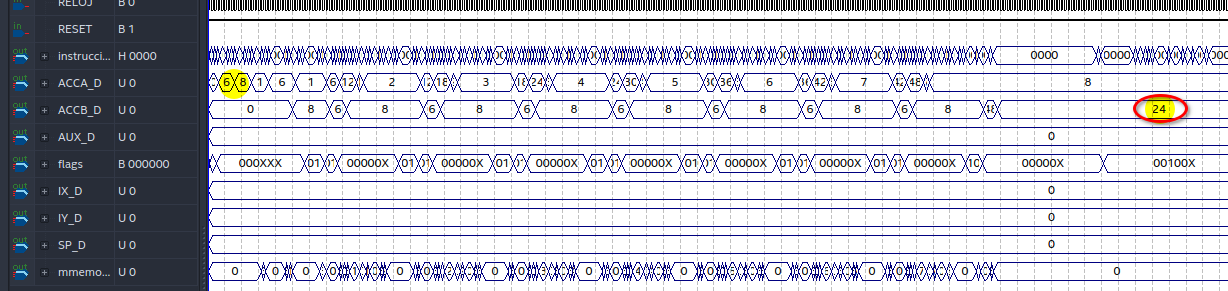
\includegraphics[width=.9\linewidth]{../img/7.png}
\caption{Resultados}
\end{figure}
\section{Conclusiones}
\label{sec:orga38d001}
\subsubsection{Romero Andrade Cristian}
\label{sec:org13c4ec7}
Se desarrolló la arquitectura Risc, donde se puede observar que la ejecución de cada instrucción es paralela, esto conlleva a una velocidad de procesamiento considerable en comparación a otras arquitecturas. sin embargo esta contiene un problema ya que tiene una dependencia de datos para cada instrucción y puede causar retrasos e inconsistencias, sin embargo esta se puede solucionar usando la operación NOP (el la práctica estas interrupciones se encarga el compilador o bien ya esta resuelta por hardware).
\section{Manual de usuario}
\label{sec:org2f4f6ab}
\subsection{Prerrequisitos}
\label{sec:orgef8bf23}
\begin{itemize}
\item Contar con Git instalado en su sistema operativo (Opcional)
\item Contar con alguno de los siguiente sistemas operativos:
\begin{itemize}
\item Windows* 10
\item Windows Server* 2012 Enterprise
\item Windows Server* 2016 Enterprise
\item Windows Server* 2019 Enterprise
\item Red Hat* Enterprise Linux* 7
\item Red Hat* Enterprise Linux* 8
\item CentOS* 7.5
\item CentOS* 8.0
\item SUSE* SLE 12
\item SUSE* SLE 15
\item Ubuntu* 16.04 LTS
\item Ubuntu* 18.04 LTS
\item Ubuntu* 20 LTS
\end{itemize}
\item El tamaño de memoria dependerá de la versión descargada
\begin{table}[htbp]
\caption{Versiónes de Quartus}
\centering
\begin{tabular}{ll}
\hline
Software & Espacio minimo\\
\hline
Quartus Prime Pro & \(20-140[GB]\)\\
Quartus Prime Standard Edition & \(15-37[GB]\)\\
Quartus Prime Lite Edition & \(14[GB]\)\\
Stand-Alone Programmer & \(3.3[GB]\)\\
Intel FPGASDK for OpenCL & \(2[GB]\)\\
Intel SoC Embedded Development Suite & \(8[GB]\)\\
Intel Advanced Link Analyzer & \(9[GB]\)\\
\hline
\end{tabular}
\end{table}
\end{itemize}
\subsection{Instalación\label{sec:instalacion}}
\label{sec:orgfd6df43}
Descargar o clonar el repositorio de \href{https://github.com/tysyak/OyAC\_Proyecto\_20221}{Github}: \href{https://github.com/tysyak/OyAC\_Proyecto\_20221}{\texttt{github.com/tysyak/OyAC\_Proyecto\_20221}}
\begin{figure}[htbp]
\centering
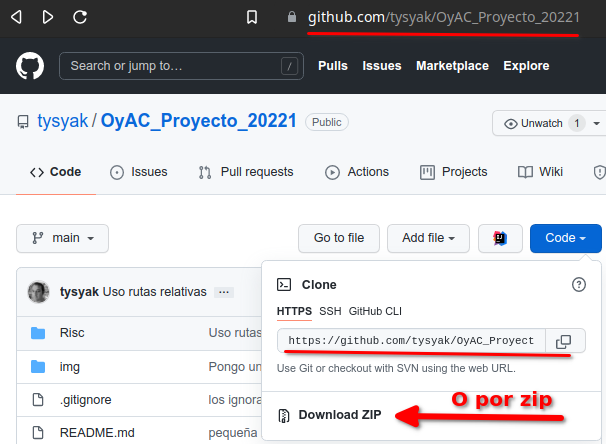
\includegraphics[width=.9\linewidth]{./img/github.png}
\caption{Repositorio del proyecto}
\end{figure}
\subsection{Uso\label{sec:uso}}
\label{sec:orgba46e7d}
\begin{enumerate}
\item Abrir Quartus Prime\footnote{A partir Quartus v21.1 modelsim es sustituido, por lo tanto la solución en la simulación vista en el presente solo sirve para versiones anteriores a 21.1}
\item En el menú File seleccionar abrir proyecto o presionar \texttt{Control + J}
\begin{center}
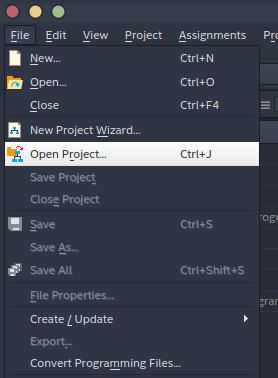
\includegraphics[width=0.6\linewidth]{../img/1.png}
\end{center}
\item Seleccionamos el proyecto (\texttt{pipeline.qpf})
\begin{center}
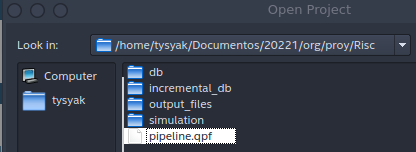
\includegraphics[width=0.6\linewidth]{../img/2.png}
\end{center}
\item Compilar el proyecto con el botón o presionando \texttt{Control + L}
\begin{center}
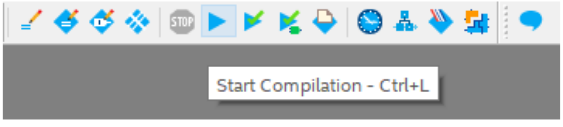
\includegraphics[width=0.6\linewidth]{./img/comp.png}
\end{center}
\item Crear un nuevo archivo
\begin{center}
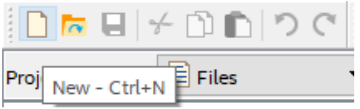
\includegraphics[width=0.6\linewidth]{./img/new1.png}
\end{center}
\item Seleccionar el tipo, \emph{University Program VWF}
\begin{center}
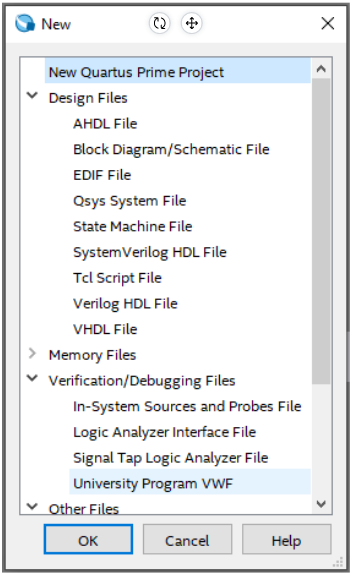
\includegraphics[width=0.6\linewidth]{./img/new2.png}
\end{center}
\item Presionar click derecho sobre el espacio blanco y seleccionar insert Node or Bus
\begin{center}
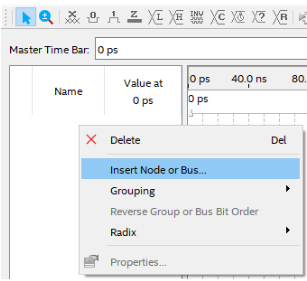
\includegraphics[width=0.6\linewidth]{./img/sim1.png}
\end{center}
\item Seleccionar Node Finder
\begin{center}
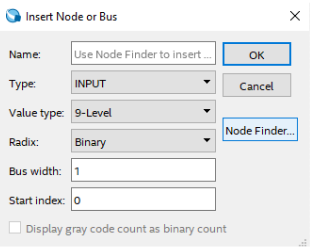
\includegraphics[width=0.6\linewidth]{./img/sim2.png}
\end{center}
\item Presionar el botón List, esto desplegara los nodos en el proyecto
\begin{center}
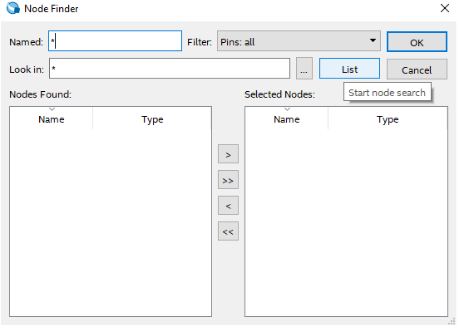
\includegraphics[width=0.6\linewidth]{./img/sim3.png}
\end{center}
\item Dar click sobre el botón \(>>\) y después dar click en el botón \textbf{OK}
\begin{center}
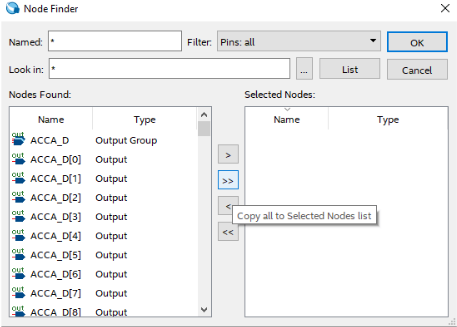
\includegraphics[width=0.6\linewidth]{./img/sim4.png}
\end{center}
\item Dar click en el botón \textbf{OK}
\begin{center}
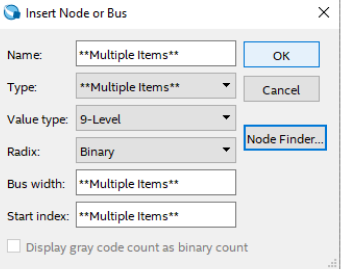
\includegraphics[width=0.6\linewidth]{./img/sim5.png}
\end{center}
\item Seleccionar el RELOJ y dar click sobre el botón 'Overwrite Clock', mostrado en la parte superior de la imagen
\begin{center}
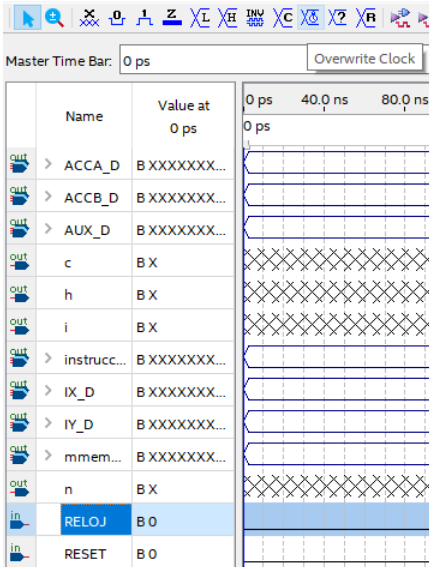
\includegraphics[width=0.6\linewidth]{./img/sim6.png}
\end{center}
\item Asignar un periodo de 5.0 y dar click sobre 'OK'.
\item Seleccionar RESET y dar click sobre el botón 'Forcing High (1)', mostrado en la parte superior de la imagen
\begin{center}
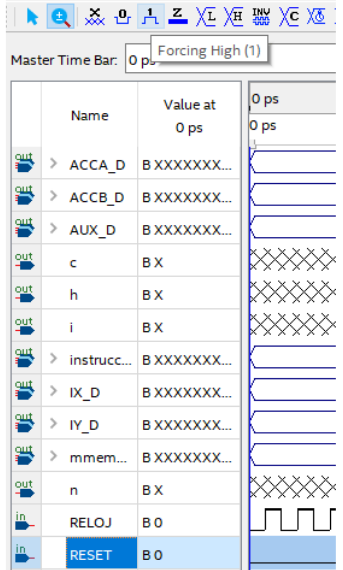
\includegraphics[width=0.6\linewidth]{./img/sim7.png}
\end{center}
\item Seleccionar del menú \emph{Simulation Settings}
\begin{center}
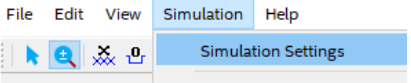
\includegraphics[width=0.6\linewidth]{./img/sim8.png}
\end{center}
\item Borrar del Script la opción \texttt{-novopt} (se muestra seleccionado en la imagen siguiente). Después presionar sobre SAVE
\begin{center}
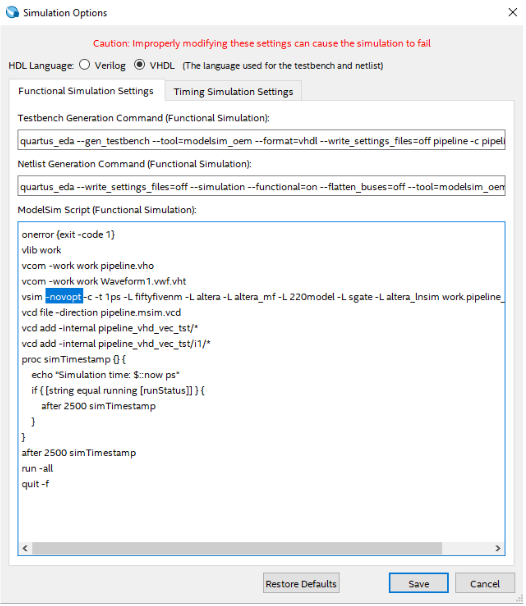
\includegraphics[width=0.6\linewidth]{./img/sim9.png}
\end{center}
\item Presionar el botón \textbf{Run Functional Simulation}
\begin{center}
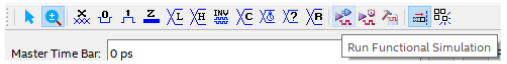
\includegraphics[width=0.6\linewidth]{./img/sim10.png}
\end{center}
\end{enumerate}

\section{Referencias}
\label{sec:orga69d27a}
\nocite{*}
\printbibliography{}

\listoffigures{}
\listoftables{}
\listoflistings{}
\end{document}
